\documentclass[a4paper,10pt]{article}
\usepackage[latin1]{inputenc}
\usepackage[swedish,english]{babel}
\usepackage{amsmath,amsthm}
\usepackage{amssymb}
\usepackage{ifpdf}
\ifpdf
  \usepackage[pdftex]{graphicx}
  \usepackage{epstopdf}
\else
  \usepackage[dvips]{graphicx}
\fi
\usepackage[margin=3.5cm]{geometry}
\usepackage[pdftitle={URDME manual},
 pdfauthor={Bauer/Drawert/Engblom/Hellander},
 pdffitwindow=true,
 breaklinks=true,
 colorlinks=true,
 urlcolor=blue,
 linkcolor=red,
 citecolor=red,
 anchorcolor=red]{hyperref}
\usepackage[sort&compress,numbers]{natbib}
\usepackage{algorithm}
\usepackage{algorithmic}

%**************************************************************************

\numberwithin{equation}{section}
\numberwithin{table}{section}
\numberwithin{figure}{section}

% function- and variable names
\newcommand{\varrs}{\texttt{urdme}}
\newcommand{\varrf}{\texttt{rdme2fem}}
\newcommand{\varfr}{\texttt{fem2rdme}}
\newcommand{\varrdme}{\texttt{rdme}}

\newcommand{\varNcells}{\texttt{Ncells}}
\newcommand{\varMspecies}{\texttt{Mspecies}}
\newcommand{\varMreactions}{\texttt{Mreactions}}
\newcommand{\varNdofs}{\texttt{Ndofs}}
\newcommand{\varM}{\texttt{M1}}
\newcommand{\vardsize}{\texttt{dsize}}
\newcommand{\varD}{\texttt{D}}
\newcommand{\varu}{\texttt{u0}}
\newcommand{\varN}{\texttt{N}}
\newcommand{\varG}{\texttt{G}}
\newcommand{\varK}{\texttt{K}}
\newcommand{\varI}{\texttt{I}}
\newcommand{\varS}{\texttt{S}}
\newcommand{\vartspan}{\texttt{tspan}}
\newcommand{\varprop}{\texttt{prop}}
\newcommand{\varreport}{\texttt{report}}
\newcommand{\varvol}{\texttt{vol}}
\newcommand{\varsd}{\texttt{sd}}
\newcommand{\vardata}{\texttt{data}}

\newcommand{\varrdmesd}{\texttt{rdme\_sd}}
\newcommand{\varrdmesdlevel}{\texttt{rdme\_sdlevel}}

\newcommand{\varU}{\texttt{U}}
\newcommand{\varfem}{\texttt{fem}}
\newcommand{\varinto}{\texttt{->}}

% variable names used in equations
\newcommand{\Ncells}{N_{\mbox{\footnotesize{cells}}}}
\newcommand{\Mspecies}{M_{\mbox{\footnotesize{species}}}}
\newcommand{\Mreactions}{M_{\mbox{\footnotesize{reactions}}}}
\newcommand{\Ndofs}{N_{\mbox{\footnotesize{dofs}}}}
\newcommand{\rand}{\mbox{rand}}

\newcommand{\fatx}{\mathbf{x}}
\newcommand{\comment}[1]{\textcolor{red}{\textbf{*** #1}}}

%**************************************************************************

\title{URDME \textit{v}. 1.2: User's manual \\}

\author{Pavol Bauer$^{\mbox{{\tiny 1}}}$ \and Brian
  Drawert$^{\mbox{{\tiny 2}}}$ \and Stefan Engblom$^{\mbox{{\tiny
        1}}}$ \and Andreas Hellander$^{\mbox{{\tiny 2}}}$}

\date{\today}

%**************************************************************************

\begin{document}
\selectlanguage{english}

\maketitle

{\footnotesize \em $^{\mbox{\tiny\rm 1}}$ Division of Scientific
  Computing, Department of Information Technology, Uppsala University,
  P.~O.~Box 337, SE-75105 Uppsala, Sweden, e-mails:
  \href{mailto:stefane@it.uu.se}{stefane@it.uu.se},
  \href{mailto:pavol.bauer@it.uu.se}{pavol.bauer@it.uu.se}.}

{\footnotesize \em $^{\mbox{\tiny\rm 2}}$ Department of Computer
  Science, University of California-Santa Barbara, Santa Barbara,
  California 93106, USA, e-mail:
  \href{mailto:bdrawert@cs.ucsb.edu}{bdrawert@cs.ucsb.edu},
  \href{mailto:andreash@cs.ucsb.edu}{andreash@cs.ucsb.edu}.}

%**************************************************************************

\medskip

{\footnotesize \textbf{Manager of this release:} Pavol Bauer (to
  whom correspondence should be addressed).}

\section{Introduction}
\label{sec:intro}

Stochastic simulation methods are frequently used to study the
behavior of cellular control systems modeled as continuous-time
discrete-space Markov processes (CTMC). Compared to the most
frequently used deterministic model, the reaction rate equations, the
mesoscopic stochastic description can capture effects from intrinsic
noise on the behavior of the networks \cite{McAdams:1999fk,
BARKAILEIBLER, Elowitz:2002fj, THATTAI, Paulsson:2000kx}.

In the discrete mesoscopic model the state of the system is the copy
number of the different chemical species and the reactions are usually
assumed to take place in a well-stirred reaction volume. The chemical
master equation is the governing equation for the probability density,
and for small to medium sized systems it can be solved by direct,
deterministic methods \cite{PaulPhD, MacThesis, Ferm:fr, SPGRIDS1,
EngSpect1, EngSpect2}. For larger models however, exact or approximate
kinetic Monte Carlo methods \cite{SSA, TAULEAP} are frequently used to
generate realizations of the stochastic process. Many different hybrid
and multiscale methods have also emerged that deal with the typical
stiffness of biochemical reactions networks in different ways, see
\cite{MSSA, nSSA, MYHYB, Rao:2003df, haseltine:6959, minlic} for examples.

Many processes inside the living cell can not be expected to be
explained in a well-stirred context. The natural macroscopic model is
the reaction-diffusion equation which has the same limitations as the
reaction rate equations. By discretizing space with small subvolumes
it is possible to model the reaction-diffusion process by a CTMC
within the same formalism as for the well-stirred case. A diffusion
event is now modeled as a first order reaction from a subvolume to an
adjacent one and the state of the system is the number of molecules of
each species in each subvolume. The corresponding master equation is
called the reaction-diffusion master equation (RDME) and due to the
very high dimensionality it cannot be solved by deterministic methods
for realistic problem sizes.

The RDME has been used to study biochemical systems in \cite{BISTAB,
MinD}. Here the next subvolume method (NSM) \cite{BISTAB}, an
extension of Gibson and Bruck's next reaction method (NRM) \cite{NRM},
was suggested as an efficient method for realizing sample
trajectories. An implementation on a structured Cartesian grid is
freely available in the software MesoRD~\cite{mesoRD}.

The method was extended to unstructured meshes in \cite{SPDEPEFHL} by
making connections to the finite element method (FEM). This has
several advantages, the most notable one being the ability to handle
complicated geometries in a flexible way. This is particularly
important in cell-biological models where internal structures often
must be taken into account.

This manual describes the software URDME which provides an efficient,
modular implementation capable of stochastic simulations on
unstructured meshes. URDME is easy to use for simulating and studying
a particular model in an applied context, but also for developing and
testing new approximate methods. We achieve this by relying on
third-party software for the geometry definition, meshing,
preprocessing and visualization, while using a highly efficient
computational core written in ANSI C for the actual stochastic
simulation. This keeps the implementation of the Monte Carlo
part small and easily expandable, while the user benefits from
the advanced pre- and post-processing capabilities of modern FEM
software. In this version of URDME, we have chosen to provide an
interface to Comsol Multiphysics 3.5a and 4.x \cite{COMSOL}.
\comment{Outdated reference! Don't find the new name...}
        
The rest of this manual is organized as
follows. Section~\ref{sec:changes} summarizes the major changes to
URDME compared to the earlier version 1.1. Section~\ref{sec:install}
describes the software requirements and the installation procedure. An
overview of the code structure is presented in Section~\ref{sec:ov2}
and the details concerning the input to the code, the provided
interface to Comsol and the way models should be specified are found
in Section~\ref{sec:details}. A URDME model is set up and simulated in
a step-by-step manner in Section~\ref{sec:ex} and in
Section~\ref{sec:integration} we show how a new core solver can be
integrated in the URDME infrastructure.

In two appendices we recapitulate the mesoscopic reaction-diffusion
model and show how the stochastic diffusion intensities are obtained
from a FEM discretization of the diffusion equation. We also list for
reference a few stochastic simulation algorithms.

We refer the interested reader to the full paper \cite{URDMEpaper} for
further information on the URDME software, including comparisons to
other available software and examples of some more advanced usage.

\section{Summary of major changes}
\label{sec:changes}

Below, we summarize the major changes compared to
URDME~1.1~\cite{URDMEman2}.
\begin{itemize}
\item URDME~1.2 includes support for Comsol~Multiphysics~4.x as well
  as Comsol~Multiphysics~3.5a. The support for
  Comsol~Multiphysics~3.5a will be removed in a coming release of
  URDME.

\item The syntax of the Matlab interface has been refined, essentially
  by moving the model-properties from \textit{fem.urdme} to the
  structure \textit{umod} and storing the Comsol Multiphysics geometry
  in the field \textit{umod.comsol}.

\item Basic SBML support has been added into URDME, allowing for
  translation of SBML level 2 files into URDME \textit{model} and
  \textit{propensity files} with the external script
  \textit{sbml2urdme}.

\item The solvers can be compiled and executed without any Matlab dependencies using a new, in-house library for reading .mat files. This feature does not support the full set of Matlab data-structures, but is compatible with the NSM and DFSP solvers. It is disabled by default. To enable it, define URDME\_LIBMAT in '/build/Makefile.nsm'. 
\item Propensities for \emph{mass-action models} can be defined directly in the Matlab model file as \emph{inline propensities}. 

\end{itemize}
 % ***
\section{Obtaining and installing URDME 1.2}
\label{sec:install}

\paragraph{Usage:}

\textit{URDME is work in progress. You may use, distribute, and
 modify the code freely under the GNU GPL license version 3. We welcome
  contributions, suggestions, comments, and bug-reports. Support questions should be directed 
  to the URDME mailing list, which you can sign up for on} \url{http://www.urdme.org}.


\subsection{System requirements and software dependencies}

\begin{itemize}
\item Linux or Apple OSX operating system.
\item Matlab
  \begin{itemize}
  \item Tested versions: 2007a, 2008a, 2008b, 2009a, 2009b, 2011b, 2012a
  \item Command line interface must be installed
  \end{itemize}
\item Comsol multiphysics 3.5a (with appropriate patches) or Comsol multiphysics 4.x
  \begin{itemize}
  \item Tested versions: 3.5a, 4.0, 4.2, 4.3 (recommended)
  \item Must have Matlab integration components installed
  \end{itemize}
\item GCC (Xcode on Apple computers, with command-line tools)
  \begin{itemize}
  \item Executables \texttt{gcc} and \texttt{make} must be in the
    path
  \item Standard libraries must be installed
  \end{itemize}
\item The optional SBML support requires additionally 
  \begin{itemize}
  \item Python runtime libraries 2.6 or higher
  \item SBML library for python (\texttt{libsbml})
  \end{itemize}
\end{itemize}

\subsection{Installation procedure}

\begin{enumerate}
\item Obtain the latest release of URDME from
  \url{https://github.com/URDME/urdme}. Download the file {\bf urdme-1.2.tar.gz}. 
\item Unpack the archive. This can be done by running the command
  ``{\bf tar -zxvf urdme-1.2.tar.gz}'' in a terminal. Often it is
  possible to double click the file icon in the operating system's
  graphical file manager.
\item Run the installation script with `system administrator'
  privileges. In a terminal, change directory to {\bf urdme-1.2}
  created from the downloaded archive. Run the script {\bf install.sh}
  with `root' or system administrator privileges. This can usually be
  done by running the command ``{\bf sudo ./install.sh}''. Follow the
  prompts of the installation script, the default values should be
  sufficient for most users. If the installation script runs with no
  errors, URDME should be installed correctly.
\end{enumerate}

\subsection{Testing of the installation {\it and} Quick start guide}
\label{sec:quickstart}

\subsubsection{Using Comsol Multiphysics 3.5}

\begin{enumerate}
\item Start Comsol and open a model file,
  e.g.~\texttt{urdme-1.2/examples/mincde/coli.mph}.
\item From Comsol, start Matlab: \\ \texttt{File >
  Client/Server/MATLAB > Connect to MATLAB}
\item Initialize the Matlab environment.
  \begin{itemize}
  \item Change Matlab's working directory to the folder for the URDME
    model you wish to simulate. At the Matlab command prompt type \\
    \texttt{>> cd urdme-1.2/examples/mincde/}
  \end{itemize}
\item Export the model geometry from Comsol to Matlab.
  \begin{itemize}
  \item Update the Model data:\\ \texttt{Solve >
    Update Model}
  \item Export the data:\\ \texttt{File > Export >
    FEM Structure as 'fem'}
  \end{itemize}
\item Simulate the model. At the Matlab command prompt
  type:\\ \texttt{>> umod = urdme(fem,'mincde')}
\item Visualize the results. At the Matlab command prompt
  type:\\ \texttt{>> postplot(umod.comsol,'Tetdata','MinD\_m')}
\end{enumerate}

\subsubsection{Using Comsol Multiphysics 4.x}

\begin{enumerate}

\item Start the Comsol interface to Matlab (''LiveLink''), \\ \texttt{./comsol server matlab} in Unix-based systems.

  \item Change Matlab's working directory to the folder for the URDME
    model you wish to simulate. At the Matlab command prompt type \\
    \texttt{>> cd urdme-1.2/examples/mincde/}

\item Load the Comsol geometry into Matlab: \\ \texttt{>> fem = mphload('coli.mph')}

\item Simulate the model. At the Matlab command prompt  type:\\ 
  \texttt{>> umod = urdme(fem,'mincde');} 

\item Visualize the results. At the Matlab command prompt type:\\ 
  \texttt{>> umod.comsol.result.create('res1','PlotGroup3D');} \\
  \texttt{>> umod.comsol.result('res1').set('t','900');} \\
  \texttt{>> umod.comsol.result('res1').feature.create('surf1', 'Surface');} \\
  \texttt{>> umod.comsol.result('res1').feature('surf1').set('expr', 'MinD\_m');} \\
  \texttt{>> mphplot(umod.comsol,'res1');} 

\item Optionally, save the output to a \textit{mph}-file for further observations in the Comsol GUI: \\
\texttt{>> mphsave(umod.comsol,'coli\_output.mph')}

\end{enumerate}

\subsubsection{Further possibilities}

To manipulate the model, edit the following files:
  \begin{description}
  \item[\texttt{coli.mph}] (Comsol model geometry, edited via the
    Comsol interface)
    \begin{itemize}
    \item[-] Physical geometry and mesh properties
    \item[-] Names of chemical species
    \item[-] Diffusion coefficients
    \end{itemize}
  \item[\texttt{mincde.m}] (Matlab pre-processing script)
    \begin{itemize}
    \item[-] Stoichiometric matrix
    \item[-] Dependency graph
    \item[-] Initial conditions of chemical species
    \item[-] Custom diffusion rules (i.e.~support for membrane-only species)
    \end{itemize}
  \item[\texttt{mincde.c}] C-functions defining the propensity (rate)
    of each reaction channel.
  \end{description}

A more detailed description on how to set up and simulate this model
is found in Section~\ref{sec:ex}.
 % xxx check
% !TEX root = manual.tex
\section{Code overview}
\label{sec:ov2}

URMDE consists of three logical layers. The top layer is made up of an
interface to an external mesh generator and pre-/post-processing
engine, currently Comsol Multiphysics. The bottom layer is a set
of simulation routines, or solvers, written in ANSI C. Interfacing
those two levels is a middle layer implemented in the Matlab
environment, designed to facilitate data processing and visualization,
as well as custom model development. Together these layers form a
software package that enables the development and efficient simulation
of complex and powerful models of spatial stochastic phenomena.

The URDME structure is designed with both efficiency and flexibility
in mind.  A model is defined by three separate files, one for each of
the logical layers. The geometry of the model is defined in a Comsol
\texttt{.mph} file, along with the names and diffusion rates of each
chemical species. A Matlab model file supplies the model with the
stoichiometric matrix, the dependency graph, and the initial state of
the system. The stoichiometric matrix defines the effect of the
chemical reactions on the state of the system while the dependency
graph indicates the reaction rates that need to be updated after a
given reaction or diffusion event has occurred. Finally, a model file
written in ANSI C specifies the propensity functions for the chemical
reactions in the system. Using compiled rather than interpreted
reaction rates ensures maximum efficiency when simulating the model.

The computational solver that ships with URDME is an efficient
implementation of NSM \cite{BISTAB}. Table~\ref{tab:code} shows the
directory structure of URDME together with a short description of each
routine.

A solver has (at least) two arguments: the path to an input file
in \texttt{.mat} format and a name of an output file on which to store
the trajectory that is generated. The input file will contain all the
data structures the solver needs, each with its specific name. The
URDME C-core contains utility routines to extract this data from the
input file.

The main steps involved in launching a solver is outlined below, along
with the routines that perform the different tasks. Generally, the
user does not have to know or perform all these steps manually: they
are all wrapped in the main routine \texttt{urdme} found in the file
`urdme.m'. However, users planning to write a plug-in solver for URDME
will benefit from a more detailed knowledge of the code structure. The
relevant steps are:

\begin{enumerate}
\item \emph{Process the \texttt{.mph} model file.}  This is achieved
  by exporting the FEM-structure from Comsol to Matlab and invoking
  the routine \texttt{comsol2urdme}. This will initialize a new structure,
  \texttt{umod} storing the original FEM-structure in the field \texttt{umod.comsol}. The
  \texttt{umod} structure contains as well the fields \varD, \varvol, \varsd, i.e.~those
  data structures related to the geometry of the model and to the
  unstructured mesh. Compare Table~\ref{tab:code}.

\item The next step is to invoke the Matlab \texttt{.m} model file to
  initialize the remaining, essential data structures, \varN, \varG,
  \varu, \vartspan\ and optionally \vardata. They should all be added
  as fields to the \texttt{umod} struct. Any modifications of the
  data structures added to the model by \texttt{comsol2urdme} in the
  previous step is typically performed in this step as well.

\item After all required fields in the \texttt{umod} struct have
  been initialized, \texttt{urdme\_validate} is invoked to perform
  error-checking on the input to make sure that all required fields in
  \texttt{umod} are present and has the correct properties.
 
\item Next, all fields in \texttt{umod} is serialized to a
  \texttt{.mat} input-file using \texttt{urdme2mat}.

\item After specifying the propensities in a ANSI C source file, the
  solver(s) are compiled using \texttt{urdme\_compile} and then
  launched by a system call from within the Matlab environment (or
  directly from e.g. a bash terminal).

\item The input file is now read by the solver, using the utility
  routine \texttt{read\_model} found in
  `matmodel.h'. \texttt{read\_model} allocates, initializes and
  returns a C-struct \texttt{urdme\_model}. This \texttt{urdme\_model}
  struct is then the sole input to the routine \texttt{nsm} found in
  `nsm.c'. \texttt{nsm} unpacks the structure and calls the main
  simulation routine \texttt{nsm\_core} found in 'nsmcore.c'. A
  similar construction should be used by contributed solvers for easy
  integration, see Section \ref{sec:integration}.

\item After successful simulation, the resulting trajectory is written
  to an output file in \texttt{.mat} format. This file is then loaded
  back into Matlab and added to the FEM-struct by
  \texttt{urdme2comsol} for visualization using Comsol routines or
  custom Matlab scripts.
\end{enumerate} 

\begin{table}[htp]
  \centering
  \begin{tabular}{|l|l|p{0.55\linewidth}|}
    \hline
    {\bf{Directory}} & {\bf{File(s)}} & {\bf{Description}} \\
    \hline
    & &\\
    bin & urdme\_init & Environmental variable helper program.\\
    & &\\
    build & Makefile & GNU Make input file for automatic solver compilation.\\
    & Makefile.nsm & Makefile for the NSM solver.\\
    & &\\
    comsol & comsol2urdme.m 
    & Matlab-script converting Comsol's FEM-struct to a valid \varrs-input. \\
    & urdme2comsol.m & Matlab-script for conversion of the output of 
    \varrs~to the solution format used by Comsol. \\
    & & \\
    doc & manual.pdf & The most recent version of this manual. \\
    & & \\
    include & matmodel.h & Functions to serialize data to/from solvers. \\
      &	propensities.h & Definition of the propensity function datatype.	\\
      & report.h     & Header for report.c. \\
     & read\_matfile.h & Functions to read/write \texttt{.mat} files.\\ 
    & & \\
    msrc  & urdme.m & Gateway routine for the solvers. \\
      & urdme\_startup.m & Initializes URDME. \\
      & urdme\_compile.m & Automatic solver compilation. \\
      & urdme\_validate.m & Input validation. \\
      & urdme2mat.m & Serialize model data for input to solvers.\\
      & urdme\_addsol.m & Read an output file and add solution to \texttt{umod}\\
      & & (used when running in background mode).\\
      & urdme\_inline\_convert.m & Convert "inline" propensities into an ANSI C propensity file.\\
    & & \\
    src & report.c &  Report function used by \varrs. \\ 
     & matmodel.c & Functions to serialize data to/from solvers.   \\ 
     & read\_matfile.c & Functions to read/write \texttt{.mat} files.\\ 
    & & \\
    src/nsm & nsm.h & Header for the NSM solver.\\
      & nsm.c & NSM solver interface.\\
      & nsmcore.c & NSM solver computational core. \\
      &	binheap.h & Header for binheap.c.\\
      & binheap.c & The binary heap used in the NSM solver.\\
    & & \\
    sbml & sbml2rdme & Translate SBML models into URDME models.\\ 
    & & \\
    examples & (various) & Contains files specifying the example
    studied in detail in Section~\ref{sec:ex}.\\
    & & \\
    \hline
  \end{tabular}
  \caption{Overview of the files and routines that make up URDME.}
  \label{tab:code}
\end{table}

 % xxx quick check
\section{Details and specifications}
\label{sec:details}

In this section we give a detailed description of the input to \varrs\
and explain how the coupling between the Comsol/Matlab interface and
the solvers works.

\subsection{Input to the solver}
\label{sec:speci}

Table~\ref{tab:rdmeinput1} summarizes the input to the NSM solver. For
precise type definitions, consult the preamble of the source file
`nsmcore.c'. While specific for the NSM solver, most of the input data
are likely to be needed by any simulation algorithm. Furthermore,
contributed solvers should preferably accept the same set of input as
the NSM solver for compatibility across models.

\begin{table}
  \begin{small}
\begin{tabular}{|l|p{0.3\linewidth}|p{0.45\linewidth}|}
  \hline
  {\bf{Name}} & {\bf{Type}} & {\bf{Description}}			\\
  \hline
    &&									\\
  \varNcells & scalar (int) & Number of subvolumes.			\\
  \varMspecies & scalar (int) & Number of different species. This 
  also defines \varNdofs $:=$ \varMspecies$\times$\varNcells.		\\
  \varMreactions & scalar (int) & Number of reactions.			\\
  \vardsize & scalar (int) & Size of the data vector used in the 
  propensity function.							\\
    &&									\\
 \varu & Matrix[\varMspecies$\times$\varNcells] (int) & \varu$(i,j)$ 
  gives the initial number of species $i$ in subvolume $j$. 		\\
  \vartspan &  vector (double) & An increasing sequence of points in 
  time where the state of the system is to be returned.			\\
  \varprop & Vector[\varMreactions] (\texttt{PropensityFun}) 
    & Propensity function pointers. See Section~\ref{sec:prop} for 
  details.								\\
  \varreport & \texttt{ReportFun} & Pointer to a report function. This 
  function is called every time the chain reaches a value in \vartspan. \\
    &&									\\
  \varvol & Vector[\varNcells] (double) 
    & The volume of the macroelements, i.e. the diagonal elements of 
    the lumped mass-matrix $M$ (cf.~Appendix~\ref{subsec:mesodiff}). \\
  \varsd &  Vector[\varNcells] (int) 
    & The subdomain numbers of all subvolumes. See Section~\ref{sec:ex} 
    for more details.							\\
  \vardata &  Matrix[\vardsize$\times$\varNcells] (double) 
    & Generalized data vector. A pointer to column $j$ is passed as an 
    additional argument to the propensities in subvolume $j$.		\\
    &&									\\
  \varD & Sparse matrix[\varNdofs $\times$ \varNdofs] (double)
    & The \emph{transpose} of the diffusion matrix $M^{-1}K$ obtained 
    from the FEM discretization of the macroscopic diffusion equation, 
    cf.~\eqref{eq:FEM}. Each column in \varD\ (i.e. each row in 
    $M^{-1}K$) corresponds to a subvolume, and the non-zero coefficients 
    $D(i,j)$ give the diffusion rate constant from subvolume $i$ to 
    subvolume $j$. 							\\
  \varN & Sparse matrix[\varMspecies\ $\times$ \varMreactions] (int) 
    & The stoichiometric matrix. Each column corresponds to a reaction, 
    and execution of reaction $j$ amounts to adding the 
    $j$th column to the state vector.					\\
  \varG & Sparse matrix[\varMreactions\ $\times$ 
    (\varMspecies+\varMreactions)] (int) 
    & Dependency graph. The first \varMspecies\ columns correspond to 
    diffusion events and the following \varMreactions\ columns to 
    reactions. A non-zeros entry in element $i$ of column $j$ indicates 
    that propensity $i$ needs to be updated if the event $j$ 
    occurs. See Section~\ref{sec:ex} for examples.			\\
 
  \hline
\end{tabular}
\caption{Input arguments to \varrs. For more details, see the source
  file `nsmcore.c'. All data in the table will be passed to the core
  simulation routine via a C-struct \texttt{urdme\_model} except
  \texttt{prop} and \texttt{report} that are specified in separate C
  files. For all sparse matrices, the compressed column sparse (CCS)
  format is used. This is the same format Matlab uses and online
  documentation is available.}
  \label{tab:rdmeinput1}
  \end{small}
\end{table}


\subsection{Specifying propensities for chemical reactions}
\label{sec:prop}

We have provided two separate methods to specify the reaction
propensities. Simple polynomial rate laws (mass-action) can be provided as inline
propensities and can be specified in the Matlab model file. For general propensities and full flexibility, the rate laws can be specified in a model file written in C.  

%The other option is to specify the rate laws in a model file written
%in C. To simplify this process, we

%Note that one can easily use \emph{both} inline and compiled
%propensities simultaneously. This is convenient when only a few
%propensities are complicated and has to be compiled.

%\subsubsection{Inline propensities}
%\label{sec:inline}

An ``inline propensity'' is a compact data format for specifying basic
chemical reactions with polynomial rate laws. An inline propensity $P$
can be defined as
\begin{align*}
  P(x) &= \left\{
 \begin{array}{rl}
    \frac{k_1x_ix_j}{\Omega}+k_2x_k+k_3\Omega & \text{if } i \ne j,	\\
    \frac{k_1x_i(x_i-1)}{2\Omega}+k_2x_k+k_3\Omega & \text{if } i = j.
  \end{array} \right.
\end{align*}
Here $x$ is the column in $\fatx$ which contains the state of the
subvolume considered and $\Omega$ is the corresponding volume. The
coefficients and indices are specified in matrices \varK\ and \varI\
where \varK$(:,r) = [k_1; \, k_2; \, k_3]$ and \varI$(:,r) = [i; \, j;
\, k]$ are the constants corresponding to the $r$th inline
propensity. The matrix \varS\ is a (possibly empty) sparse matrix such
that \varS$(:,r)$ lists all subdomains in which the $r$th inline
propensity is turned off. \emph{Note that no inline propensities are
active in subdomain zero!} A complete example of the use of inline propensities can be found in the 'annihilation' example that ships with URDME 1.2. 



%\subsubsection{Compiled propensities}
%\label{sec:compiled}

The other (and fully general way) to specify propensity functions are
to supply them to \texttt{urdme} as a model file written in ANSI
C. The precise form of the propensity functions is defined by the data
type \texttt{PropensityFun}, defined in the header `propensities.h'
(found in the `include' directory) as

\begin{verbatim}
typedef double (*PropensityFun)(const int *x, double t, double vol, 
                                const double *data, int sd);
\end{verbatim}

The arguments \varvol, \vardata, and \varsd\ to a
\texttt{PropensityFun} are described in
Table~\ref{tab:rdmeinput1}. Additionally, the input vector \texttt{x}
of length \varMspecies\ is the copy number in a given subvolume, and
\texttt{t} is the absolute time. Note that none of the current solvers
are capable of simulating Markov chains with explicitly time-dependent
propensities. The time argument is included in the typedef at this
stage only to simplify future developments.
 
Below is a commented example of a model file defining a simple
chemical system composed of a single species $X$ undergoing a
dimerization reaction.

\begin{verbatim}
/* Propensity definition of a simple dimerization reaction. */
#include <stdlib.h>
#include <stdio.h>
/* Type definition for propensity functions: */
#include "propensities.h"

/* Rate constant. */
const double k = 1.0e-3;

double rFun1(const int *x, double t, double vol, const double *data, int sd)
/*  X + X -> 0. */
{
  return k*x[0]*(x[0]-1)/vol;
}

PropensityFun *ALLOC_propensities(void)
/* Allocation. */
{
  PropensityFun *ptr = (PropensityFun *)malloc(sizeof(PropensityFun));
  ptr[0] = rFun1;

  return ptr;
}

void FREE_propensities(PropensityFun *ptr)
/* Deallocation. */
{
  free(ptr);
}

\end{verbatim}
\noindent
A model file \emph{must} implement the following routines:
\begin{itemize}
  \item \verb#PropensityFun *ALLOC_propensities(void)#
  \item \verb#void FREE_propensities(PropensityFun *ptr)#
\end{itemize}

\noindent
The first function should allocate and initialize an array of function
pointers to the propensity functions and return a pointer to this
array. This is the function that the solvers will call to access the
rate functions.  The second function should deallocate the pointer
\texttt{ptr}. For further examples, see Section \ref{sec:ex}.
 % xxx check
\section{Using the SBML interface}
\label{sec:sbml}
The SBML interface is found in the \texttt{sbml} directory and allows for translation of downloaded SBML files to URDME
compatible model and propensity definitions.

\subsection{Installation procedure}

\begin{enumerate}

\item Install the Python runtime libraries (Version 2.6 or higher)
available at \url{http://www.python.org}.

\item Download and install the official SBML library from \url{http://sbml.org/Software/libSBML}.
Make sure to enable the language interface (API) to Python during the installation.  The detailed guide on
how to compile \textit{libsbml} with the Python API is available in the online documentation of the library.

\end{enumerate}

\subsection{Testing and quick start guide}

\begin{enumerate}

\item Change into the \texttt{sbml} directory of the URDME installation. 

\item You can now use the \texttt{sbml2urdme} translator to generate a propensity and model function
of the \textit{mincde} example, described in detail in chapter \ref{sec:ex}.
Execute the bash-script \texttt{sbml2rdme} in combination with the provided SBML-file \texttt{mincde.xml} as first parameter.

\texttt{./sbml2rdme mincde.xml}

You should obtain the following information:

\texttt{Creating model c-file mincde.c} \\
\texttt{Creating model m-file mincde.m}

\item The script generated a model (.m) and propensity (.c) file with the same filename as the
SBML specification file (in this case 'mincde'). You can proceed with execution the generated files
together with geometries imported from Comsol Multiphysics. \\
\texttt{umod = urdme(fem,'mincde')}

Asuming the geometry definition to be available in the variable \texttt{fem}.

  \smallskip 
   
  {\bf \textcolor{red}{!}} The SBML Level 2 specification is not sufficient to describe all properties and dynamics
  of a full URDME model. Although the generated models are fully operational they can be considered
  as drafts which can be manually extended with more specific model requirements. See chapter \ref{sec:ex} for extensions
  of the \textit{mincde}-model.

\end{enumerate}

\subsection{Usage guide}
The SBML translator can be called as a bash-script where \texttt{model.xml} is the SBML definition file and the 
output directory is an optional parameter. \\

\texttt{./sbml2rdme <model.xml> [output directory]} \\

Alternatively, the Python script \texttt{sbml2rdme.py} available in  \texttt{sbml/src} directory of the distribution
can be called with the same parameters within the Python environment.

\subsection{Limitations}
In the actual version the translator supports exclusively SBML Level 2. Reverse reactions are not supported.
 
\section{Example: Min oscillations in \emph{E. Coli}}
\label{sec:ex}

In this section we describe the general workflow involved in setting up and
simulating a model in URDME using the Comsol and Matlab
interfaces. The major steps are:

\begin{enumerate}
\item \emph{Specify the model}. This involves defining the geometry,
  mesh, initial conditions and chemical reactions of the model. In
  URDME, this will require the generation of three model
  files: a Comsol model file `model.mph' , a Matlab model file
  `model.m' and a reaction propensity ANSI C file `model.c', where we use
  {\it model} as a placeholder for the non-extension part of the
  file-name.
  
  The Comsol model defines the geometric domain of the problem and
  Comsol Multiphysics is used to create a mesh representing the
  spatial discretization of the diffusion equation with Neumann
  boundary conditions and the corresponding inter-voxel diffusion jump
  coefficients. The Matlab model file specifies the chemical reaction
  networks of the problem by defining a stoichiometric matrix
  \varN\ and a dependency graph \varG. The propensity functions for
  the chemical reactions are specified in the ANSI C model file.
	
\item \emph{Export the FEM-structure from Comsol to Matlab.} After
  defining the geometry and using Comsol to create a tetrahedral mesh
  of the model, the resulting data structure (FEM) is exported from
  Comsol to the Matlab workspace via the built-in Comsol/Matlab
  coupling.
	
\item \emph{Run the simulation.} The solver is launched from the
  Matlab workspace via the interface routine in `urdme.m'. As input,
  you will have to specify the \texttt{.m} and \texttt{.c} model
  files. Internally, \texttt{urdme} uses \texttt{comsol2urdme} to
  initialize the main structure \texttt{umod}.The function defined in the 
  file `model.m' file then appends data to this structure.
  	
\item \emph{Post-processing.} After a normal termination of the
  solver, a trajectory of the stochastic process will be attached to
  the Comsol file stored in \texttt{umod.comsol}. At this point, you can use all post-processing
  options available in the Comsol interface to visualize the results. If you have
  other needs not covered by the built-in routines, you can implement
  your own post-processing scripts in Matlab. If using Comsol Multiphysics 4.x, you
  might as well save the solution stored in \texttt{umod.comsol} to a file via the command \textit{mphsave}
  and observe0 it externally in the Comsol GUI.
\end{enumerate}
 
To illustrate the above steps in detail, we will reproduce simulations
of the Min system from \cite{MinD}. The geometry will be a model of an
\emph{E.~coli} bacterium. It is rod shaped with length $3.5\mu m$ and
diameter $0.5\mu m$. The reactions and parameters of the model can be
found in Table\ \ref{tab:MinD}.

\begin{table}[htp]
\centering
\begin{tabular}{ll}
  $\mbox{MinD\_c\_atp} \xrightarrow{k_d} \mbox{MinD\_m}$ & 
  $\mbox{MinD\_c\_atp}+\mbox{MinD\_m} \xrightarrow{k_{dD}} \mbox{2MinD\_m} $ \\
  $\mbox{Min\_e+MinD\_m} \xrightarrow{k_{de}} \mbox{MinDE}$ & 
  $\mbox{MinDE} \xrightarrow{k_e} \mbox{MinD\_c\_adp} + \mbox{Min\_e} $ \\
  $\mbox{MinD\_c\_adp} \xrightarrow{k_p} \mbox{MinD\_c\_atp}$
 \end{tabular} 
  \caption{The chemical reactions of the MinD/MinE model. The
    constants take the values $k_d = 0.0125\mu m^{-1}s^{-1}$, $k_{dD}
    = 9 \times 10^6 M^{-1}s^{-1}$, $k_{de} = 5.56\times 10^7
    M^{-1}s^{-1}$, $k_e=0.7s^{-1}$ and $k_p = 0.5s^{-1}$.}
  \label{tab:MinD}
\end{table}

\subsection{Setting up the model for simulation}

The following steps shows how to create the Comsol model file. If you
don't want to go through all the steps yourself, open the example file
`coli.mph' in the `examples/mincde' folder.

\paragraph*{Defining the geometry and diffusion rates in Comsol Multiphysics 3.5}

\begin{enumerate}
\item Open Comsol and select `Chemical engineering module -- Mass
  transport -- Diffusion -- Transient analysis' (3D). In the
  `Dependent variables' field write \texttt{MinD\_c\_atp MinD\_m,
  Min\_e MinDE MinD\_c\_adp}. These are the names of the variables
  that we will use. Select \emph{Lagrange -- Linear} elements and
  press `OK'.
  
    {\bf \textcolor{red}{!}} \emph{Note that the `Chemical engineering module' is not required 
    in general for URDME, but is used in this example for convenience.}


  \item Next we create the geometry. We will build the rod shaped
  domain from two spheres and one cylinder. Press the `Cylinder'
  button and in the radius and height field enter \texttt{0.5e-6} and
  \texttt{3.5e-6} and press `OK'. You should now see a cylinder in
  your workspace. In the `Draw mode' action bar, press `Zoom extents'
  in order to get a better view of the domain.  Press the `sphere'
  button and enter \texttt{0.5e-6} in the radius field and press
  `OK'. Create another identical sphere but enter \texttt{3.5e-6} as
  the $z$-coordinate. Select all three figures and press the `union'
  button and then the `Delete interior boundaries' button.

\item Having defined the species and the geometry, the next step is to
  specify the parameters in the model. In the menu `Physics $>$
  Subdomain settings', choose subdomain 1 and set the diffusion
  constants to \texttt{2.5e-12} for \texttt{MinD\_c\_adp,
    MinD\_c\_atp} and \texttt{Min\_e}. For \texttt{MinDE} and
  \texttt{MinD\_m} the diffusion constant should be \texttt{1e-14}.
  
  \smallskip 
   
  {\bf \textcolor{red}{!}} \emph{\texttt{MinDE} and \texttt{MinD\_m}
    are membrane bound species, hence their lower diffusion rates. We
    have not specified this explicitly at this stage, but will do so
    later in the \texttt{Matlab} model file.}

\item In order to be able to distinguish between the interior of the
  bacterium and the membrane, we must also create two domains. One
  interior domain that represents the cytoplasm and one boundary
  domain that represents the membrane. This is done by defining the
  special variable \varrdmesd\ as an expression with different value
  in the different subdomains. It can then be used to distinguish the
  nodes on the boundary from those in the interior. Select `Options
  $>$ Subdomain expressions' and enter \varrdmesd\ with value 1 and
  click `OK'. Select `Options $>$ Boundary expressions' and select all
  boundaries (there should be 12 of them). Enter \varrdmesd\ with
  value 2. Finally select `Options $>$ Global expressions' and enter
  \varrdmesdlevel\ with value 2 indicating that the \emph{lowest}
  dimension where \varrdmesd\ is defined is on the surface of the
  geometry.

\item In the `Mesh' menu, select `Mesh $>$ Free mesh parameters' and
  choose `Custom mesh size'.  Set the maximum element size to
  \texttt{1e-7} and press `Initialize mesh'.  Now select `Solve $>$
  Update model'.  Make sure that you are connected to Matlab, if not,
  connect via `File $>$ Client/Server/Matlab $>$ Connect to MATLAB'.
  Then export the FEM structure to the Matlab workspace from the `File
  $>$ export' menu.
\end{enumerate}

\paragraph*{Defining the geometry and diffusion rates in Comsol Multiphysics 4.x}

\begin{enumerate}
\item Open Comsol and use the Model Wizard to create the model template.
Select `3D' as space dimension' and add the physics module `Chemical Species Transport / Transport of Diluted Species' 
in the next step. In the `Dependent variables' window chose the `Number of species' to be \texttt{5}
and in the `Concentrations' list enter the names \texttt{MinD\_c\_atp MinD\_m,
  Min\_e MinDE} and  \texttt{MinD\_c\_adp}. These are the names of the variables
  that we will use.  Select the `Time Dependent' study type in the next step of the wizard and click 
  on the flag symbol to create the template.
  
    {\bf \textcolor{red}{!}} \emph{Note that the `Chemical engineering module' is not required 
    in general for URDME, but is used in this example for convenience.}

\item Next we create the geometry. We will build the rod shaped
  domain from two spheres and one cylinder. Right click on `Geometry 1', 
  select the `Cylinder' option and in the radius and height field enter \texttt{0.5e-6} and
  \texttt{3.5e-6}. Click on the `Build Selected' Button and you should now see a cylinder in
  your workspace. 
  Now, select the `Sphere' node from the `Geometry' context-menu and and enter 
  \texttt{0.5e-6} in the radius field. Create another identical sphere but enter \texttt{3.5e-6} as
  the $z$-coordinate.  Click on `Build All' and observe the created domain in the graphics-window.
  
  Right click on `Geometry' again and select `Boolean Operations $>$ Union'. Select all three
  domains and add them to the `Input objects' selection.  Uncheck the `Keep interior boundaries'
  box and complete the geometry creation by pushing the `Build All' button.

\item Having defined the species and the geometry, the next step is to
  specify the parameters in the model. In the physics settings  `Transport of Diluted Species $>$
  Transport Mechanisms', deactivate the flag on `Convection'.
  Next we need to specify the diffusion constants of the species in the `Diffusion' node of the physics menu.
  Enter the diffusion coefficients \texttt{2.5e-12} for \texttt{MinD\_c\_adp,
    MinD\_c\_atp} and \texttt{Min\_e}. For \texttt{MinDE} and
  \texttt{MinD\_m} the diffusion constant should be \texttt{1e-14}. The units of all constants are $m^2/s$.
  
  \smallskip 
   
  {\bf \textcolor{red}{!}} \emph{\texttt{MinDE} and \texttt{MinD\_m}
    are membrane bound species, hence their lower diffusion rates. We
    have not specified this explicitly at this stage, but will do so
    later in the \texttt{Matlab} model file.}

\item In order to be able to distinguish between the interior of the
  bacterium and the membrane, we must also create two domains. One
  interior domain that represents the cytoplasm and one boundary
  domain that represents the membrane. This is done by defining the
  special variable \varrdmesd\ as an expression with different value
  in the different subdomains. It can then be used to distinguish the
  nodes on the boundary from those in the interior. 
  
  Click right on the menu `Definitions', and create two `Variables' elements.
  In the first one, select the `Geometry entity level' to be `Domain' and chose
  the `Selection' to be `All domains'.  Now, enter a new variable in the window below
  by specifying the name to \texttt{rdme\_sd} and expression to \texttt{1}.
  
  In the second Variable-element, specify the geometric entity level to `Boundary'
  and set the `Selection' to `All boundaries'. Enter the variable name \texttt{rdme\_sd} into
  the `Variables' window and set the expression to \texttt{2} indicating that the \emph{lowest}
  dimension where \varrdmesd\ is defined is on the surface of the
  geometry.

\item In the `Mesh' node, set `User controlled mesh' as sequence type and
  in the appeared `Size' node select the `Custom' option.  Set the maximum element size to
  \texttt{1e-7} and press `Build All'.  Now click on the `Study' node and press the `Compute' button.  
  
  Now you need to transfer the created geometry into Matlab. Make sure that you are connected to the Server, if not,
  connect via `File $>$ Client Server $>$ Connect to Server'.
  When having a working connection the export can be performed by selecting `File $>$ Client Server $>$ Export Model to Server'.
  
  Another option is to save the model as a \textit{mph-file}, and open it later in a  running Matlab
  session with `LiveLink' via the command \texttt{mphload}.
\end{enumerate}

\paragraph*{Specifying the chemical reactions}

The chemical reactions are specified in a separate model file written
in C. This file will be given as input to URDME, which will compile
and launch a solver. Every time the reaction propensity file is
changed, the solver needs to be recompiled, but this will be
automatically detected by URDME.  The way the reaction propensity
functions are specified are explained in more detail in Section
\ref{sec:prop}, which we recommend that you read before continuing
with this example.

The following code specifies the reaction propensity model \texttt{.c}
file for the reactions in Table \ref{tab:MinD}. This file is located
in `examples/mincde/fange.c' in the URDME installation
directory. Either open that file, or create a new one of your own,
entering the code below.

%/* Ordering of the species. */
%const enum {MinD_c_atp = 0,
%            MinD_m     = 1,
%            MinD_e     = 2,
%            MinDE      = 3,
%            MinD_c_adp = 4};

%/* Indicator values of sd. */
%const enum {CYTOSOL = 1, MEMBRANE = 2};

%/* Number of reactions. */
%const int NR = 5;

\begin{verbatim}

#include <stdlib.h>
#include "propensities.h"

/* Ordering of the species. */
#define MinD_c_atp 0
#define MinD_m     1
#define MinD_e     2
#define MinDE      3
#define MinD_c_adp 4

/* Indicator values of sd. */
#define CYTOSOL  1
#define MEMBRANE 2

/* Number of reactions. */
#define NR       5

/* Rate constants. */
const double NA    = 6.022e23;
const double kd    = 1.25e-8;
const double kdd   = 9.0e6; 
const double kde   = 5.56e7;
const double ke    = 0.7;
const double k_adp = 1.0;

/* Reaction propensities. */
double rFun1(const int *x, double t, double vol, const double *data, int sd)
/* MinD_c_atp -> MinD_m */
{
  if (sd == MEMBRANE) 
    return kd*x[MinD_c_atp]/data[0];
  return 0.0;
}

double rFun2(const int *x, double t, double vol, const double *data, int sd)
/* MinD_c_atp + MinD_m -> 2MinD_m */
{
  return kdd*x[MinD_c_atp]*x[MinD_m]/(1000.0*NA*vol);
}

double rFun3(const int *x, double t, double vol, const double *data, int sd)
/* MinD_m + Min_e -> MinDE */
{
  return kde*x[MinD_m]*x[MinD_e]/(1000.0*NA*vol);
}

double rFun4(const int *x, double t, double vol, const double *data, int sd)
{
  return ke*x[MinDE];
}

double rFun5(const int *x, double t, double vol, const double *data, int sd)
/* MinD_c_adp -> MinD_c_atp */
{
   return k_adp*x[MinD_c_adp];
}


PropensityFun *ALLOC_propensities(void)
{
  PropensityFun *ptr = malloc(sizeof(PropensityFun)*NR);
  
  ptr[0] = rFun1;
  ptr[1] = rFun2;
  ptr[2] = rFun3;
  ptr[3] = rFun4;
  ptr[4] = rFun5;

  return ptr;
}

void FREE_propensities(PropensityFun* ptr)
{
  free(ptr);
}
\end{verbatim}

\noindent
There are a few points that deserves highlighting:

\begin{itemize}
\item Note the unit conversions given explicitly in the bimolecular
  propensity function. The rate constants for the bimolecular
  reactions in this model are given in the unit $M^{-1}s^{-1}$ and
  need to be converted to mesoscopic rates. That is why we divide with
  Avogadros number times the volume of the subvolume. Also, the way we
  have set up the geometry model file, the volume is given in the unit
  $m^3$, and needs to be converted to $L^3$. URDME cannot keep track
  of matching the units between the different model files
  automatically: this is the responsibility of the end-user.

\item Note how we use the input \texttt{sd} in the first reaction to
  make sure that it only occurs in subvolumes lying on the
  membrane. We have to make sure, however, that we keep track of what
  value we assigned to the different subdomains in the Comsol model
  file (the value of the expression \texttt{rdme\_sd}).

\item The input \texttt{t} passes the current time to the propensity
  function. This input is included in the typedef of the propensity
  function to make it more general and accommodate future
  needs. However, the NSM-solver does not currently handle time dependent
  propensities correctly. 
  %While an explicitly time dependent  propensity will not generate any run-time errors, 
  Thus, the resulting
  stochastic trajectory will not be a statistically correct
  realization of the intended process.

\item The first reaction in the model contains a scaling with the
  local length scale of the subvolume. For a uniform Cartesian mesh
  this would simply have been the (constant) side lengths of the cubes
  in the mesh. For the unstructured mesh however, this value will be
  different in every subvolume. It is readily obtained from Comsol,
  and is passed to the propensity function via the data vector
  \vardata. \vardata\ will be initialized with the correct values in
  the Matlab model file \texttt{fange.m}, next to be described.
\end{itemize}

\paragraph*{Creating a .m model file}

Before we can run the simulation, we have yet to specify a few more
data structures. We will also need to modify the diffusion rates that
we obtain from the initial Comsol model so that the membrane-bound
species only diffuse on the membrane. We have already prepared for
this by labeling the subvolumes next to the boundary using the
expression \texttt{rdme\_sd} in the Comsol model file `coli.mph'.

Open the file `examples/mincde/fange.m'. We will walk through the
contents of this file and explain what the different parts
do. Additional information can also be found in the comments in the
file.

\begin{enumerate}

\item \emph{The stoichiometric matrix.} To execute the reactions, the
  solvers need to know the stoichiometry of the reactions. This is
  specified via a sparse matrix \varN\ of dimensions
  \varMspecies\ $\times$ \varMreactions. Entry $(i,j)$ in \varN\ tells
  how species $i$ changes upon execution of reaction $j$. The
  following lines of code will set up the stoichiometric matrix for
  our example:

\begin{verbatim}
% Stoichiometric matrix. Every column corresponds to a reaction.
umod.N = sparse([-1  -1  0  0  1 ;...
                  1   1 -1  0  0 ;...
                  0   0 -1  1  0 ;...
                  0   0  1 -1  0 ;...
                  0   0  0  1 -1]);
                
\end{verbatim} 

\item \emph{The dependency graph.} Efficient implementations of
  simulators for large systems uses a dependency graph to minimize the
  re-computation of rates. URDME requires that such a graph \varG, in
  the form of a sparse matrix, be submitted to the NSM-solver. It
  should have dimensions \varMreactions\ $\times$
  (\varMspecies+\varMreactions). The following code sets up \varG\ for
  this example.

\begin{verbatim}
% Dependency graph. The first Mspecies columns indicate the propensities
% that need to be updated when the corresponding species diffuses. The 
% next Mreactions columns work analogously for reaction events.
umod.G = sparse([1 0 0 0 0 1 1 0 0 1;...
                 1 1 0 0 0 1 1 1 0 1;...
                 0 1 1 0 0 1 1 1 1 0;...
                 0 0 0 1 0 0 0 1 1 0;...
                 0 0 0 0 1 0 0 0 1 1;]);
\end{verbatim}

A non-zero entry at row $i$ in column $j$ means that propensity number
$i$ must be updated if species $j$ diffuses ($j \leq $ \varMspecies)
or if reaction $j-$\varMspecies\ occurs ($j > $ \varMspecies).

{\color{red}{{\bf !}}} \emph{A common reason for errors when
  developing a new model is errors in \varN\ or \varG}. A quick way of
setting up the dependency graph is \texttt{umod.G =
  sparse(ones(Mreactions, Mspecies+Mreactions))}. This will make all
propensities be recomputed after each event. While making the code run
slower, this is guaranteed to be correct and can be useful when
debugging your model file.

\item \emph{The initial condition.} There is complete freedom in
  specifying the initial condition. In the present case we simply
  distribute 4002 $MinD\_c\_{atp}$ and 1040 $MinE$ molecules in some
  random way in the entire bacterium.

%\begin{verbatim}
%% Specify the total number of molecules of the species. 
%nMinD = 4002;
%nMinE = 1040;

%u0 = zeros(Mspecies,Ncells);

%% random index to nMinD subvolumes
%ind = floor(NCells*rand(1,nMinD))+1;

%% use sparse to accumulate
%u0(5,:) = full(sparse(1,ind,1,1,Ncells));

%% analogously
%ind = floor(Ncells*rand(1,nMinE))+1;
%u0(3,:) = full(sparse(1,ind,1,1,Ncells));

%fem.urdme.u0 = u0;
%\end{verbatim}
\begin{verbatim}
% Specify the total number of molecules of the species. 
nMinD = 4002;
nMinE = 1040;

u0 = zeros(Mspecies,Ncells);

ind = floor(Ncells*rand(1,nMinE))+1;
u0(3,:) = full(sparse(1,ind,1,1,Ncells));

ind = floor(Ncells*rand(1,nMinD))+1;
u0(5,:) = full(sparse(1,ind,1,1,Ncells));

umod.u0 = u0;
\end{verbatim}

  Note that the code above does not produce a uniformly random initial
  distribution since the volume of each voxel is not taken into
  account.

\item \emph{Specifying the times to output the state of the system.}
  URDME will look for a vector \texttt{tspan} to determine when to
  output the state of the trajectory (the number of events generated
  in a typical realization often exceeds $10^9$ so we can't output
  after each event). Here, we want to sample the system on the time
  interval $[0,200s]$, with output each second. This is achieved by:

\begin{verbatim}
umod.tspan = 0:200. 
\end{verbatim}
 
 \item \emph{Membrane diffusion}. In order to make $MinD\_m$ and
   $MinDE$ diffuse only on the membrane, we will zero out all elements
   in the diffusion matrix that are in the cytosol. To obtain indices
   of those subvolumes we use the information in the \emph{subdomain
     vector} \texttt{sd}. \texttt{sd} will be generated by the
   \varrs\ interface upon calling the solver interface, and will
   contain the information encoded in the expression \texttt{rdme\_sd}
   in the Comsol model file. For more details, see Section
   \ref{sec:details}.

\begin{verbatim}
pm  = find(umod.sd == 2);
cyt = find(umod.sd == 1);
\end{verbatim} 
 
  Remember that we gave \texttt{rdme\_sd} the value 2 on the membrane
  and 1 in the interior. The diffusion matrix \texttt{D} will contain
  the rate constants for the diffusive events on the unstructured
  mesh. \texttt{D} is also generated from the Comsol model file when
  calling the solver, and will be available to the .m model file in
  \texttt{umod.D}. To (efficiently) zero out the correct entries
  in \texttt{D}, we first decompose the sparse matrix, find the
  entries using \texttt{pm} and \texttt{cyt} above, and then
  reassemble the matrix again (compensating for the removed entries by
  adjusting the diagonal of the matrix).  All in all, the code to do
  this is as follows:

\begin{verbatim}
% For MinD_m (2) and MinDE (4), flag all dofs in the cytosol for 
% removal. 
ixremove = [];
for s = [2 4]
  ixremove = [ixremove; Mspecies*(cyt-1)+s];
end

D = umod.D';

% Decompose the sparse matrix. 
[i,j,s] = find(D);

% Set all elements in the diffusion matrix corresponding 
% to the cytosol to zero.
ixremove = [find(ismember(i,ixremove)); find(ismember(j,ixremove))];
i(ixremove) = [];
j(ixremove) = [];
s(ixremove) = [];

% Reassemble the sparse matrix and adjust the diagonal entries. 
ixkeep = find(s > 0);
D = sparse(i(ixkeep),j(ixkeep),s(ixkeep),Ndofs,Ndofs);
d = full(sum(D,2));
D = D+sparse(1:Ndofs,1:Ndofs,-d);

umod.D = D';
\end{verbatim}

 {\color{red}{\bf !}} \emph{It is of fundamental importance that the
   columns of \texttt{D} sum to zero, and that all off-diagonal
   entries are positive. For an introduction to how \texttt{D} is
   constructed, see Appendix \ref{app:coeffs}. For a detailed account,
   consult \cite{SPDEPEFHL}}.
 
 {\color{red}{\bf !}} \emph{The way we have modeled membrane diffusion
   is simply by saying that the subvolumes closest to the membrane
   constitute the membrane layer. As the mesh becomes finer near the
   boundary, the thickness of this layer will decrease, eventually
   approaching a 2D model of the membrane. One can think of other ways
   of modeling the membrane diffusion. The most obvious is to
   explicitly draw the membrane as a separate (true) subdomain with a
   fixed thickness in the Comsol model file. This would usually mean
   that more subvolumes are needed to resolve that thin layer.}
 
 \item \emph{The generalized data vector.} Finally, we need to set
   \texttt{umod.data} to contain the values of the length
   parameter for the subvolumes (it is needed in the first reaction,
   \texttt{rFun1}). To do this, we use the built-in Comsol function
   \texttt{postinterp} in version 3.5 or \texttt{mphinterp} in version 4.x 
   which can be used to evaluate an expression in
   any point in the domain. Here, we simply get the subvolume sizes by
   using the pre-defined expression \emph{h}, evaluated in the
   vertices of the mesh.

When using Comsol Multiphysics 3.5 we type:
\begin{verbatim}
dofs = xmeshinfo(fem,'Out','dofs');
umod.data = postinterp(umod.comsol,'h',dofs.coords(:,1:Mspecies:end));
umod.data = umod.data(dofs.nodes(1:Mspecies:end));
\end{verbatim}

In Comsol Multiphysics 4.x we use the following code instead:
\begin{verbatim}
xmi = mphxmeshinfo(umod.comsol);
umod.data = mphinterp(umod.comsol,'h','coord', ...
xmi.dofs.coords(:,1:Mspecies:end), 'solnum', 1);
umod.data = umod.data(xmi.dofs.nodes(1:Mspecies:end)+1);
\end{verbatim}

{\color{red}{\bf !}} \emph{The ordering of the vertices in the mesh 
 in the FEM structure (e.g.\ \texttt{fem.mesh.p}) is not necessarily the same as the ordering in 
 Comsol's extended mesh format of the degrees of freedom.  To ensure that the ordering is consistent 
 between these two structures we can alternatively transform them using the following method in Comsol 3.5:}

\begin{verbatim}
dofs = xmeshinfo(fem,'Out','dofs');
data = postinterp(fem,'h',fem.mesh.p); 
umod.data = data(dofs.nodes(1:Mspecies:end));
\end{verbatim}

\emph{For more details concerning the internal ordering of the dofs,
  consult the Comsol user's manual. The interface routines
  \texttt{comsol2urdme} and \texttt{urdme2comsol} also contain useful
  information on this matter. }

%\emph{Note that the subdomain data vector \varsd\ is a completely 
%general piece of information. In particular, it need not be explicitly
%related to the `subdomain' numbers in \Comsol.}

\end{enumerate}

\subsection{Running the simulation}

With all three model files set up correctly, we are now ready to
launch the simulation. In Matlab, change the current working directory
to `examples/mincde' (or if you have prepared your files in another
directory, to that one). 

First, we need to load the Comsol Multiphysics FEM-model into the Matlab
workspace, either by requesting it from the server or by typing:

\begin{verbatim}
>> fem = mphload('coli.mph');
\end{verbatim}

Asuming \texttt{coli.mph} is the file name of the model previously created in Comsol Multiphysics.
To launch the simulation, call the main interface routine in `urdme.m':

\begin{verbatim}
>> umod = urdme(fem,'mincde');
\end{verbatim}

URDME will now extract information from the Comsol and Matlab model
files, compile the solver with linking to the propensities specified in
\texttt{mincde.c}, and then execute the solver by making a system call.

\subsection{Post-processing}

If the simulation in the previous step completed without errors, the
model structure will now contain a realization of the stochastic
process. To visualize the trajectory, we can use any of the
visualization options available in Comsol or we can create routines of
our own. To look at the \texttt{MinD\_m} distribution on the membrane
at the final time we can use Comsol's post-processing functionality:

\paragraph*{Post-processing using Comsol Multiphysics 3.5}

\begin{verbatim}
>> postplot(umod.comsol,'Tetdata','MinD_m');
\end{verbatim} 

To visualize the result at any other time, e.g after 100s:
\begin{verbatim}
>> postplot(umod.comsol,'Tetdata','MinD_m','T',100);
\end{verbatim}

 {\color{red}{\bf {!}}} \emph{You can specify any time in the interval
   you simulated, but if you specify a time that lies between two
   points in \texttt{tspan} Comsol will do interpolation to
   approximate the result at that point.}

\noindent
To visualize a species inside the domain, we can do as follows:

\begin{verbatim}
>> postplot(umod.comsol,'Slicedata','MinD_c_atp');
\end{verbatim} 

\noindent
There are many more options that can be passed to \texttt{postplot} to
control the plot produced. For a detailed account , see the Comsol
documentation:
\begin{verbatim}
>> help postplot
\end{verbatim}

\noindent
If you prefer to work within the Comsol GUI for visualization, you can
import the FEM structure stored in \texttt{umod.comsol} with the attached stochastic trajectory back
into Comsol. 

\noindent
Then, from the Comsol GUI, import the new structure (umod.comsol): 'File $>$
Import $>$ FEM structure...'. You can now visualize the trajectory
using the menu 'Postprocessing $>$ Plot Parameters'.
\paragraph*{Post-processing using Comsol Multiphysics 4.x} 

\begin{verbatim}
>> umod.comsol.result.create('res1','PlotGroup3D');
\end{verbatim} 

This command creates a plot-contanainer for the following visualization. \\

To visualize the result at a specific time, e.g after 100s:

\begin{verbatim}
>> umod.comsol.result('res1').set('t','100');
\end{verbatim}

 {\color{red}{\bf {!}}} \emph{You can specify any time in the interval
   you simulated, but if you specify a time that lies between two
   points in \texttt{tspan} Comsol will do interpolation to
   approximate the result at that point.} \\

\noindent

To visualize the result of the simulation on the surface we can use:

\begin{verbatim}
>> umod.comsol.result('res1').feature.create('surf1', 'Surface');
>> umod.comsol.result('res1').feature('surf1').set('expr', 'MinD_m');
>> mphplot(umod.comsol,'res1');
\end{verbatim}

Where we can replace the string \texttt{'MinD\_m'} with the name of any other occupied species. \\

To visualize the solution inside the domain, we need to first create a new plot container.

\begin{verbatim}
>> umod.comsol.result.create('res2', 'PlotGroup3D');
>> umod.comsol.result('res2').set('t','100');
\end{verbatim} 

Now we can visualize the solution on a `slice' of the $zx$-axis of the model.

\begin{verbatim}
>> umod.comsol.result('res2').feature.create('slc2', 'Slice');
>> umod.comsol.result('res2').feature('slc2').set('expr', 'MinD_c_atp');
>> umod.comsol.result('res2').feature('slc2').set('quickplane', 'zx');
>> umod.comsol.result('res2').feature('slc2').set('quickynumber', '1');
>> mphplot(model,'res2');
\end{verbatim} 

\noindent
There are many more options that can be passed to \texttt{postplot} to
control the plot produced. For a detailed account, see the Comsol
documentation:
\begin{verbatim}
>> help mphplot
\end{verbatim}

\noindent
If you prefer to work within the Comsol GUI for visualization, you can
import the FEM structured with the attached stochastic trajectory back
into Comsol. This can be done by typing:

\begin{verbatim}
>> mphsave(umod.comsol,'output_filename.mph')
\end{verbatim}

\noindent
Optionally, from the Comsol GUI, import the new structure (umod.comsol): 'File $>$
Client Server  $>$ Import Model from Server'. You can now visualize the trajectory
using the options provided in the `Results' node.
 % *** 
\section{Integrating solvers with URDME}
\label{sec:integration}

In this section we will describe how to integrate a third party
spatial stochastic solver into URDME using the DFSP \cite{DFSP} plugin
as an example. URDME plugins have three main components: the makefile,
the solver executable, and (optionally) a pre-execution script. Each
part is described in Table~\ref{tab:dfspIntgration} where the files
that make up the DFSP solver are explained. We recommend that
developers follow this format when integrating their own solvers.

\begin{table}[htb!]
  \centering
  \begin{tabular}{|l|l|p{0.55\linewidth}|}
    \hline
    {\bf{Directory}} & {\bf{File(s)}} & {\bf{Description}}\\
    \hline
    & & \\
    build & Makefile.dfsp & Solver makefile, for building the 
    solver automatically when calling \varrs.  The name of this file
    is very important: the automatic compilation process looks for a
    makefile that is suffixed with the name of the solver (in lower
    case).  This makefile compiles the solver with the model's
    propensity functions into the low-level executable which is called
    by the middle-level interface. \\
    & & \\
    src/dfsp & dfsp.c & Solver entry point and data initialization
    code. Contains a \texttt{main}-function and setup routines for
    the data structures. The initialization procedure takes the
    \texttt{.mat} file (which is a serialization of the
    \texttt{umod} structure from the Matlab workspace) and
    instantiates a \texttt{urdme\_model} struct (defined in
    include/matmodel.h). \\
    & dfsp.h & Header file containing all function prototypes
    necessary for DFSP. \\
    & dfspcore.c & Main entry point for the solver: the function 
    \texttt{dfsp\_core}. \\
    & dfsp\_reactions.c & Helper function to process reaction events.\\
    & dfsp\_diffusion.c & Helper function to process diffusion events.\\
    & & \\
    msrc & urdme\_init\_dfsp.m & Pre-execution script to initialize
    data structures before the solver is called.  When executing a
    model with a specified solver, the URDME-interface looks for a
    Matlab-function named \texttt{urdme\_init\_}$<$solver$>$ (that is,
    in the file `urdme\_init\_$<$solver$>$.m'). \\
    \hline
  \end{tabular}
  \caption{Overview of the files that make up the DFSP plugin solver.}
  \label{tab:dfspIntgration}
\end{table}

When the middle level interface calls the solver executable, it passes
all model and geometry data to the solver via a \texttt{.mat} data
file. The names of the input file and the output file are both
specified as command line arguments (i.e.~in the \texttt{argv}
parameter to the \texttt{main} function). The core URDME distribution
includes routines to read and parse this data file into a C-language
struct (see the header file `matmodel.h').  The solver is then called
with the model struct as a parameter.  Once the solver has finished
simulating the model, it attaches the calculated solution trajectory
to the model structure. The solution trajectory is then serialized to
the output file using supplied routines (see `urdme.m').  When the
solver has completed its execution, the middle level interface imports
the serialized solution trajectory and makes it
available to the post-processing and visualization routines. The
logical separation of solvers from the rest of the URDME software
enables streamlined development and debugging of new computational
methods.

For efficient simulation of URDME models, it is necessary to compile
the model specific propensity functions with the routines of the
solver chosen to perform the simulation.  The solver specific
makefiles are responsible for this compilation.  For illustration we
will use the DFSP plugin and the ``mincde'' model as an example
(i.e.~replace `dfsp' with the name of the solver you wish to
integrate). From the middle-level Matlab interface, when the
\texttt{urdme} function is called with the parameter
\texttt{\{'Solver','dfsp'\}}, URDME attempts to compile the executable
`urdme/fange.dfsp' from the propensity function file `fange.c' and
solver files using the compilation specified in `Makefile.dfsp' in
`urdme/build'. The makefile is responsible for all necessary steps of
the compilation process and the target executable is built in the
`urdme' subdirectory of the current working directly, and is named
according to the propensity file (`fange.c') and solver DFSP, thus
`urdme/fange.dfsp'. The automatic compilation process is designed
for ease of use from the middle-level Matlab interface.

Often spatial stochastic simulation methods require additional
processing of geometry and model data before execution can proceed.
In URDME, this is accomplished through the use of a specifically named
Matlab function found in the `urdme/msrc' subdirectory of the URDME
distribution.  For the DFSP plugin, this file is named
`urdme\_init\_dfsp.m'. The function defined in this file must take as
arguments the \texttt{fem} data structure and a variable number of
additional arguments (i.e.~\texttt{varargin}). If \texttt{urdme} is
called with solver arguments, that cell-vector is passed as the second
argument to this function. Implementation of a pre-processing script
provides method developers with a powerful and flexible way to perform
any necessary data transformations for their specific solvers.
 % xxx quick check
\section*{Acknowledgment}

The authors are grateful to Per L{\"o}tstedt and Linda Petzold for
valuable input during the development of URDME.

\paragraph{Previous contributor:} Josef Cullhed (v.~1.0).

\paragraph{Funding:} 

The Linnaeus center of excellence UPMARC, Uppsala Programming for
Multicore Architectures Research Center (PB, SE). U.S.~NIH grant
R01EB7511, U.S.~DOE award DE-FG02-04ER25621, U.S.~NSF IGERT
DGE-02-21715 and grant DMS-1001012, Institute for Collaborative Biotechnologies Grant
W911NF-09-0001 from the U.S.~Army Research Office (BD), U.S.~ National Institute of Biomedical Imaging And Bioengineering of the National Institute of Health under Award Number R01-EB014877-01 (BD, AH) The Swedish Graduate School in Mathematics and Computing (SE, AH), the Royal Swedish Academy of Sciences scholarship
FOA08H-109, FOA09H-63, FOA09H-64, SSF A3 02:124 (AH).

The content is solely the responsibility of the authors and does not necessarily
represent the official views of these agencies.  %required for some funding agencies


 % xxx quick check

\bibliographystyle{plain}
\newpage
\bibliography{manual}
\clearpage

\appendix
 \section{Stochastic chemical kinetics}
\label{app:coeffs}
 
 In this section we briefly describe how reaction and diffusion events
are modeled and how we obtain the diffusion rate constants when the
domain is discretized using an unstructured mesh. For a more detailed
introduction to the subject along with many additional references,
consult e.g. \cite{stefan_phd}.

The computational core of URDME is based on the next subvolume method
(NSM) \cite{BISTAB}. Details
concerning the actual simulation algorithms can be found in
Appendix~\ref{app:algorithms}.


\subsection{Mesoscopic chemical kinetics}

In a well-stirred chemical environment reactions are understood as
transitions between the states of the integer-valued state space
counting the number of molecules of each of $D$ different species. The
intensity of a transition is described by a \emph{reaction propensity}
defining the transition probability per unit of time for moving from
the state $x$ to $x+N_r$;
\begin{align}
  \label{eq:prop}
  x &\xrightarrow{\omega_{r}(x)} x+N_{r},
\end{align}
where $N_{r} \in \mathbf{Z}^{D}$ is the transition step and is the
$r$th column in the \emph{stoichiometric matrix}
$N$. Eq.~\eqref{eq:prop} defines a continuous-time Markov chain over
the positive $D$-dimensional integer lattice.

When the reactions take place in a container of volume $\Omega$, it is
sometimes useful to know that the propensities often satisfy the
simple scaling law
\begin{align}
  \omega_{r}(x) &= \Omega u_{r}(x/\Omega)
\end{align}
for some function $u_{r}$ which does not involve $\Omega$. Intensities
of this form are called \emph{density dependent} and arise naturally
in a variety of situations \cite[Ch.~11]{Markovappr}.

\subsection{Mesoscopic diffusion}
\label{subsec:mesodiff}

In the mesoscale model, a diffusion event is modeled as a first order
reaction taking species $S_l$ in subvolume $\zeta_i$ from its present
subvolume to an adjacent subvolume $\zeta_j$,
\begin{equation}
  S_{li} \xrightarrow{a_{ij}\fatx_{li}} S_{lj},
\end{equation}        
where $\fatx_{li}$ is the number of molecules of species $l$ in
subvolume $i$. On a uniform Cartesian mesh such as those used in
MesoRD \cite{mesoRD}, the rate constant takes the value $a_{ij}=\gamma
/h^2$ where $h$ is the side length of the subvolumes and $\gamma$ is
the diffusion constant. In URDME we use an unstructured mesh made up
of tetrahedra and the rate constants are taken such that the expected
value of the number of molecules divided by the volume (the
concentration) converges to the solution obtained from a consistent
FEM discretization of the diffusion equation
\begin{equation}
  u_t = \gamma \Delta u.
\end{equation}
Using piecewise linear Lagrange elements and mass lumping, we obtain
the discrete problem
\begin{equation}
  \label{eq:FEM}
  u_t = M^{-1}Ku
\end{equation}
where $M$ is the lumped mass matrix and $K$ is the
stiffness matrix. The rate constants on the unstructured mesh are then
given by
\begin{equation}
  a_{ij} = \frac{1}{\Omega_i} k_{ij}, 
\end{equation}
where $\Omega_i$ is the diagonal entry of $M$ and can be interpreted
as the volume of the dual element associated with mesh node $i$ (see
Figure~\ref{fig:dual}). For more details, consult
\cite{SPDEPEFHL}.

\begin{figure}[htb!]
  \centering  
  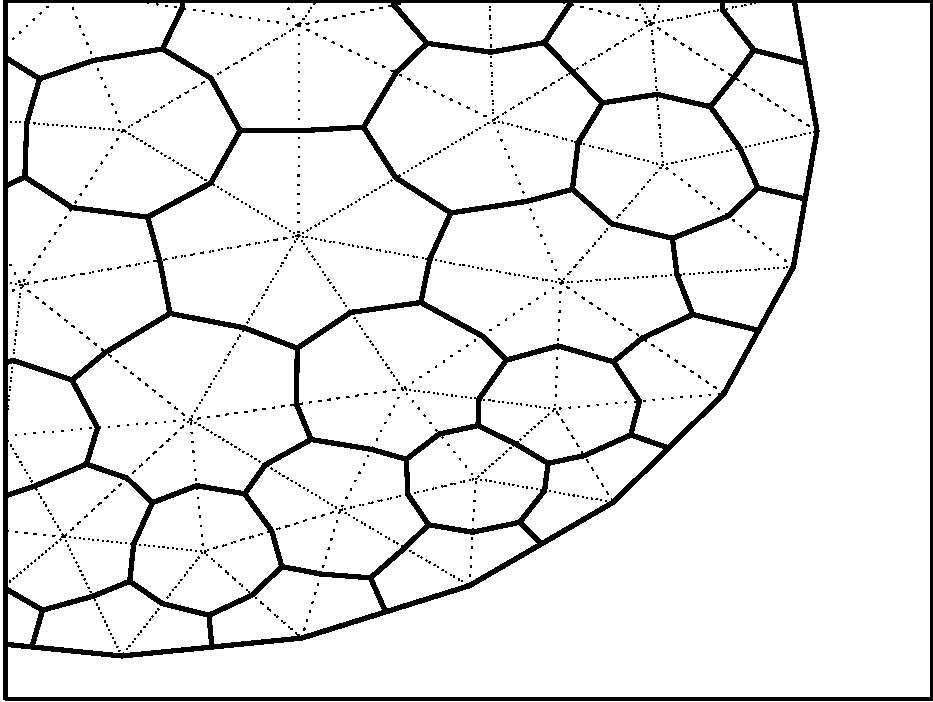
\includegraphics[width=0.6\linewidth,height=0.6\linewidth]
    {fig/URDMEmesh}
  \caption{A 2D example of an unstructured triangular mesh. The primal
  mesh is shown in dashed and the dual in solid. Within each dual
  element the system is assumed to be well-stirred, and molecules can
  jump from each dual cell to the neighboring ones.}
  \label{fig:dual}
\end{figure}

The assumption made in the mesoscopic model is that molecules are
well-stirred within a dual cell. These dual cells correspond to the
cubes of the staggered grid in a Cartesian mesh.

\section{Algorithms}
\label{app:algorithms}

One of the most popular algorithms to generate realizations of the
CTMC in the well-stirred case is Gillespie's direct method (DM)
\cite{SSA}. Several algorithmic improvements of this method exist,
one of them being the next reaction method (NRM) due to Gibson and
Bruck \cite{NRM}.

The underlying algorithm in URDME is the next subvolume method (NSM)
\cite{BISTAB}. The NSM can be understood as a combination of NRM and
DM in order to tailor the algorithm to reaction-diffusion processes.

For reference, we first state below both DM and NRM and then outline
NSM.

\begin{algorithm}[htb!]
\caption{Gillespie's direct method (DM)}
\begin{algorithmic}
  \STATE{\textit{Initialize:} Set the initial state $\fatx$ and
  compute all propensities $\omega_r(\fatx), r=1, \ldots,
  \Mreactions$. Also set $t=0$.}

  \WHILE{$t < T$}

  \STATE{Compute the sum $\lambda$ of all the propensities.}

  \STATE{Sample the next reaction time (by inversion), $\tau = -
  \log(\rand)/\lambda$. Here and in what follows, `$\rand$'
  conveniently denotes a uniformly distributed random number in
  $(0,1)$ which is different for each occurrence.}
  
  \STATE{Sample the next reaction event (by inversion); find $n$ such
  that \newline $\sum_{j=1}^{n-1} \omega_j(\fatx) < \lambda \, \rand
  \le \sum_{j=1}^n \omega_j(\fatx)$}

  \STATE{Update the state vector, $\fatx = \fatx+N_n$ and set
  $t=t+\tau$.}

  \ENDWHILE

\end{algorithmic}
\label{alg:SSADM}
\end{algorithm}

\begin{algorithm}[htb!]
\caption{Gibson and Bruck's next reaction method (NRM)}
\begin{algorithmic}
  \STATE{\textit{Initialize:} Set $t = 0$ and assign the initial
  number of molecules. Generate the dependency graph $G$. Compute the
  propensities $\omega_{r}(\fatx)$ and generate the corresponding
  \emph{absolute} waiting times $\tau_{r}$ for all reactions
  $r$. Store those values in a heap $H$.}

  \WHILE{$t < T$}

  \STATE{Remove the smallest time $\tau_{n} = H_{0}$ from the top of
  $H$, execute the $n$th reaction $\fatx := \fatx+N_{n}$ and set $t :=
  \tau_{n}$.}

  \FORALL{edges $n \to j$ in $G$}

  \IF{$j \not = n$}

  \STATE{Recompute the propensity $\omega_{j}$ and update
    the corresponding waiting time according to
\begin{align*}
  \tau_{j}^{\mathrm{new}} &= t+\left(\tau_{j}^{\mathrm{old}}-t\right)
  \frac{\omega_{j}^{\mathrm{old}}}{\omega_{j}^{\mathrm{new}}}.
\end{align*}}

  \ELSE[$j = n$]

  \STATE{Recompute the propensity $\omega_{n}$ and generate a new
  absolute time $\tau_{n}^{\mathrm{new}}$. Adjust the contents of $H$
  by replacing the old value of $\tau_{n}$ with the new one.}

  \ENDIF

  \ENDFOR

  \ENDWHILE
\end{algorithmic}
\label{alg:NRM}
\end{algorithm}

\begin{algorithm}[htb!]
\caption{The next subvolume method (NSM)}
\label{alg:NSM}
\begin{algorithmic}
  \STATE{\textit{Initialize:} Compute the sum $\sigma_i^r$ of all
  reaction rates $\omega_{ri}$ and the sum $\sigma_i^d$ of all
  diffusion rates $a_{ij}\fatx_{si}$ in all subvolumes $i=1,\ldots
  ,\Ncells$. Compute the time until the next event in each subvolume,
  $\tau_i = -\log(\rand)/(\sigma_i^r+\sigma_i^d)$, and store all times
  in a heap $H$.}

  \WHILE{$t < T$}

  \STATE{Select the next subvolume $\zeta_n$ where an event takes
  place by extracting the minimum $\tau_n$ from the top of $H$.}
  
  \STATE{Set $t=\tau_n.$} 

  \STATE{Determine if the event in $\zeta_n$ is a reaction or a
  diffusion event. Let it be a reaction if $(\sigma_n^r+\sigma_n^d) \,
  \rand < \sigma_n^r$, otherwise it is a diffusion event.}

  \IF{Reaction event}
  
  \STATE{Determine the reaction channel that fires. This is done by
  inversion of the distribution for the next reaction given $\tau_n$
  in the same manner as in Gillespie's direct method in
  Algorithm~\ref{alg:SSADM}.}

  \STATE{Update the state matrix using the (sparse) stoichiometric
    matrix $N$.}

  \STATE{Update $\sigma_n^r$ and $\sigma_n^d$ using the dependency
  graph $G$ to recalculate only affected reaction- and diffusion
  rates.}

  \ELSE[Diffusion event]

  \STATE{Determine which species $S_{ln}$ diffuses and subsequently,
  determine to which neighboring subvolume $\zeta_{n'}$. This is
  again done by inversion using a linear search in the corresponding
  column of $D$.}

  \STATE{Update the state: $S_{nl}=S_{nl}-1$, $S_{n'l}=S_{n'l}+1$.}
  
  \STATE{Update the reaction- and diffusion rates of subvolumes
  $\zeta_n$ and $\zeta_{n'}$ using G.}
  
  \ENDIF
  
  \STATE{Compute a new waiting time $\tau_n$ by drawing a new random
  number and add it to the heap $H$.}
  
  \ENDWHILE 
\end{algorithmic}
\end{algorithm}



\end{document}

%**************************************************************************
